\documentclass[a4paper,oneside]{ctexbook}
\usepackage{gbt7714}
\bibliographystyle{gbt7714-numerical}
\usepackage{geometry}
 \geometry{
 a4paper,
 total={170mm,257mm},
 left=20mm,
 top=20mm,
 }
\usepackage{graphicx}
\usepackage{subcaption}
\usepackage{indentfirst}
\usepackage{graphicx}
\graphicspath{ {./src/} }
\usepackage{hyperref}
\hypersetup{
    colorlinks=true,
    linkcolor=blue,
    filecolor=magenta,
    urlcolor=cyan,
}
\usepackage{longtable}
\usepackage{hhline}
\usepackage{booktabs}
\usepackage{makecell}
\usepackage{multirow}
\usepackage{array}
\usepackage{ragged2e}
\newcolumntype{R}[1]{>{\RaggedLeft\arraybackslash}p{#1}}
\newcommand\VRule[1][\arrayrulewidth]{\vrule width #1}
\usepackage{listings}
\usepackage{xcolor}

\definecolor{codegreen}{rgb}{0,0.6,0}
\definecolor{codegray}{rgb}{0.5,0.5,0.5}
\definecolor{codepurple}{rgb}{0.58,0,0.82}
\definecolor{backcolour}{rgb}{0.95,0.95,0.92}

\lstdefinelanguage{JavaScript}{
  keywords={typeof, new, true, false, catch, function, return, null, catch, switch, var, if, in, while, do, else, case, break},
  keywordstyle=\color{blue}\bfseries,
  ndkeywords={class, export, boolean, throw, implements, import, this},
  ndkeywordstyle=\color{darkgray}\bfseries,
  identifierstyle=\color{black},
  sensitive=false,
  comment=[l]{//},
  morecomment=[s]{/*}{*/},
  commentstyle=\color{purple}\ttfamily,
  stringstyle=\color{red}\ttfamily,
  morestring=[b]',
  morestring=[b]"
}

\lstdefinestyle{mystyle}{
    backgroundcolor=\color{backcolour},   
    commentstyle=\color{codegreen},
    keywordstyle=\color{magenta},
    numberstyle=\tiny\color{codegray},
    stringstyle=\color{codepurple},
    basicstyle=\ttfamily\small,
    breakatwhitespace=false,         
    breaklines=true,                 
    captionpos=b,                    
    keepspaces=true,                 
    numbers=left,                    
    numbersep=5pt,                  
    showspaces=false,                
    showstringspaces=false,
    showtabs=false,                  
    tabsize=2
}

\lstset{style=mystyle}

\begin{document}

\clearpage
%% temporary titles
% command to provide stretchy vertical space in proportion
\newcommand\nbvspace[1][3]{\vspace*{\stretch{#1}}}
% allow some slack to avoid under/overfull boxes
\newcommand\nbstretchyspace{\spaceskip0.5em plus 0.25em minus 0.25em}
% To improve spacing on titlepages
\newcommand{\nbtitlestretch}{\spaceskip0.6em}
\pagestyle{empty}
\begin{center}
    \bfseries
    \nbvspace[1]
    \Huge
    {\nbtitlestretch\huge
        图书管理系统}

    \nbvspace[1]
    \normalsize

    Project 5 实验报告\\
    数据库系统 (2024年\ 春夏学期)\\
    浙江大学
    \nbvspace[1]
    \\%\small BY\\
    \Large 姓名\\[0.5em]
    \footnotesize 学号\\
    指导教师: 苗晓晔

    \nbvspace[2]
    完成日期: 2024 年 5 月 10 日
    \nbvspace[3]
    \normalsize

    Made\\
    \large
    With \LaTeX
    \nbvspace[1]
\end{center}

\tableofcontents

\chapter{简介}

\section{实验目标}

完成基本实验及 Bouns 前后端。

\section{实验环境}

\begin{itemize}
    \item 服务器:
    \begin{itemize}
        \item 类型:阿里云轻量应用服务器
        \item 配置:2核4GB
        \item 操作系统:Debian 11
        \item 数据库:MySQL Community Server 8.4.0
        \item 前端:Node.js 20.13.0
        \item 前端页面地址:
        \item 后端:OpenJDK 17.0.11
        \item 后端 API 地址:
    \end{itemize}
    \item 本地开发环境:
    \begin{itemize}
        \item 操作系统:macOS 14.5
        \item IDE:IntelliJ IDEA 2023.3.4
    \end{itemize}
\end{itemize}

\chapter{系统设计及实现}

\section{图书管理系统 E-R 图}

\begin{figure}[h!]
    \centering
    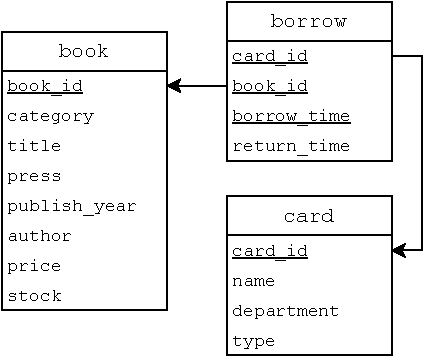
\includegraphics[width=0.5\textwidth]{e-r}
    \caption{图书管理系统 E-R 图}
    \label{fig:e-r}
\end{figure}

\section{正确性部分:主要函数设计思路}

正确性部分主要实现 \verb|LibraryManagementSystemImpl.java| 中的函数,具体要求已在接口定义文件中给出。实现每个函数的步骤基本相同:

\begin{itemize}
    \item 阅读接口要求,构造 SQL 语句
    \item 使用 JDBC 创建相应的 \verb|PreparedStatement|
    \item 从函数调用参数中获取参数,设置 \verb|PreparedStatement| 的参数
    \item 执行 SQL 语句
    \item 根据 SQL 语句的执行结果,返回相应的 \verb|ApiResult|
\end{itemize}

作为示例,代码清单~\ref{lst:incbook}~是图书存量增加函数的代码:

\begin{lstlisting}[language=java, caption=增加图书存量函数,label=lst:incbook]
@override
public ApiResult incBookStock(int bookId, int deltaStock) {
    Connection conn = connector.getConn();
    try {
        // make sure stock is always non-negative
        PreparedStatement stmt = conn.prepareStatement("SELECT stock FROM book WHERE book_id = ?");
        stmt.setInt(1, bookId);
        ResultSet rs = stmt.executeQuery();
        if (!rs.next()) {
            return new ApiResult(false, "Book not found");
        }
        int stock = rs.getInt("stock");
        if (stock + deltaStock < 0) {
            return new ApiResult(false, "Stock will be negative");
        }
        // update stock
        stmt = conn.prepareStatement("UPDATE book SET stock = stock + ? WHERE book_id = ?");
        stmt.setInt(1, deltaStock);
        stmt.setInt(2, bookId);
        stmt.executeUpdate();
        commit(conn);
    } catch (Exception e) {
        rollback(conn);
        LOGGER.log(Level.SEVERE, e.getMessage());
        e.printStackTrace();
        return new ApiResult(false, e.getMessage());
    }
    return new ApiResult(true, null);
}
\end{lstlisting}

对于并发请求部分,我选择的方法是将隔离级别设置为 \verb|TRANSACTION_SERIALIZABLE|,这是最高级别的隔离。这意味着每个事务都完全与其他事务隔离,就好像它们是串行执行的一样。

\begin{lstlisting}[language=java, caption=并发请求处理]
public ApiResult borrowBook(Borrow borrow) {
    conn.setTransactionIsolation(Connection.TRANSACTION_SERIALIZABLE);
}
\end{lstlisting}

所实现的程序通过了所有测试,结果如图~\ref{fig:test-pass}~所示:

\begin{figure}[!h]
    \centering
    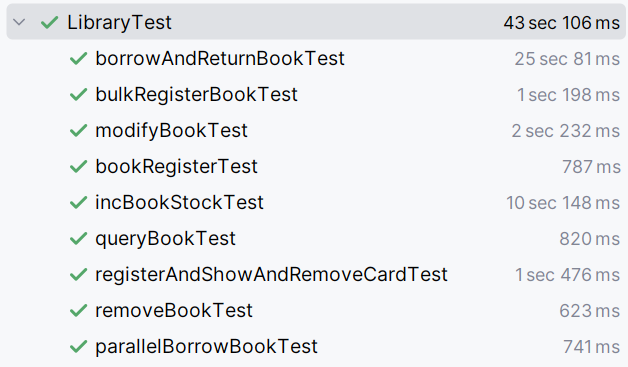
\includegraphics[width=0.5\textwidth]{test.png}
    \caption{通过测试截图}
    \label{fig:test-pass}
\end{figure}

\section{功能性部分:前端设计思路}

前端采用 Vue + Element-UI 库实现,按照实验指导中的思路结合个人审美,最终设计出的前端界面如下三图所示:

\begin{figure}[ht]
    \centering
    \begin{subfigure}{.5\linewidth}
       \centering
       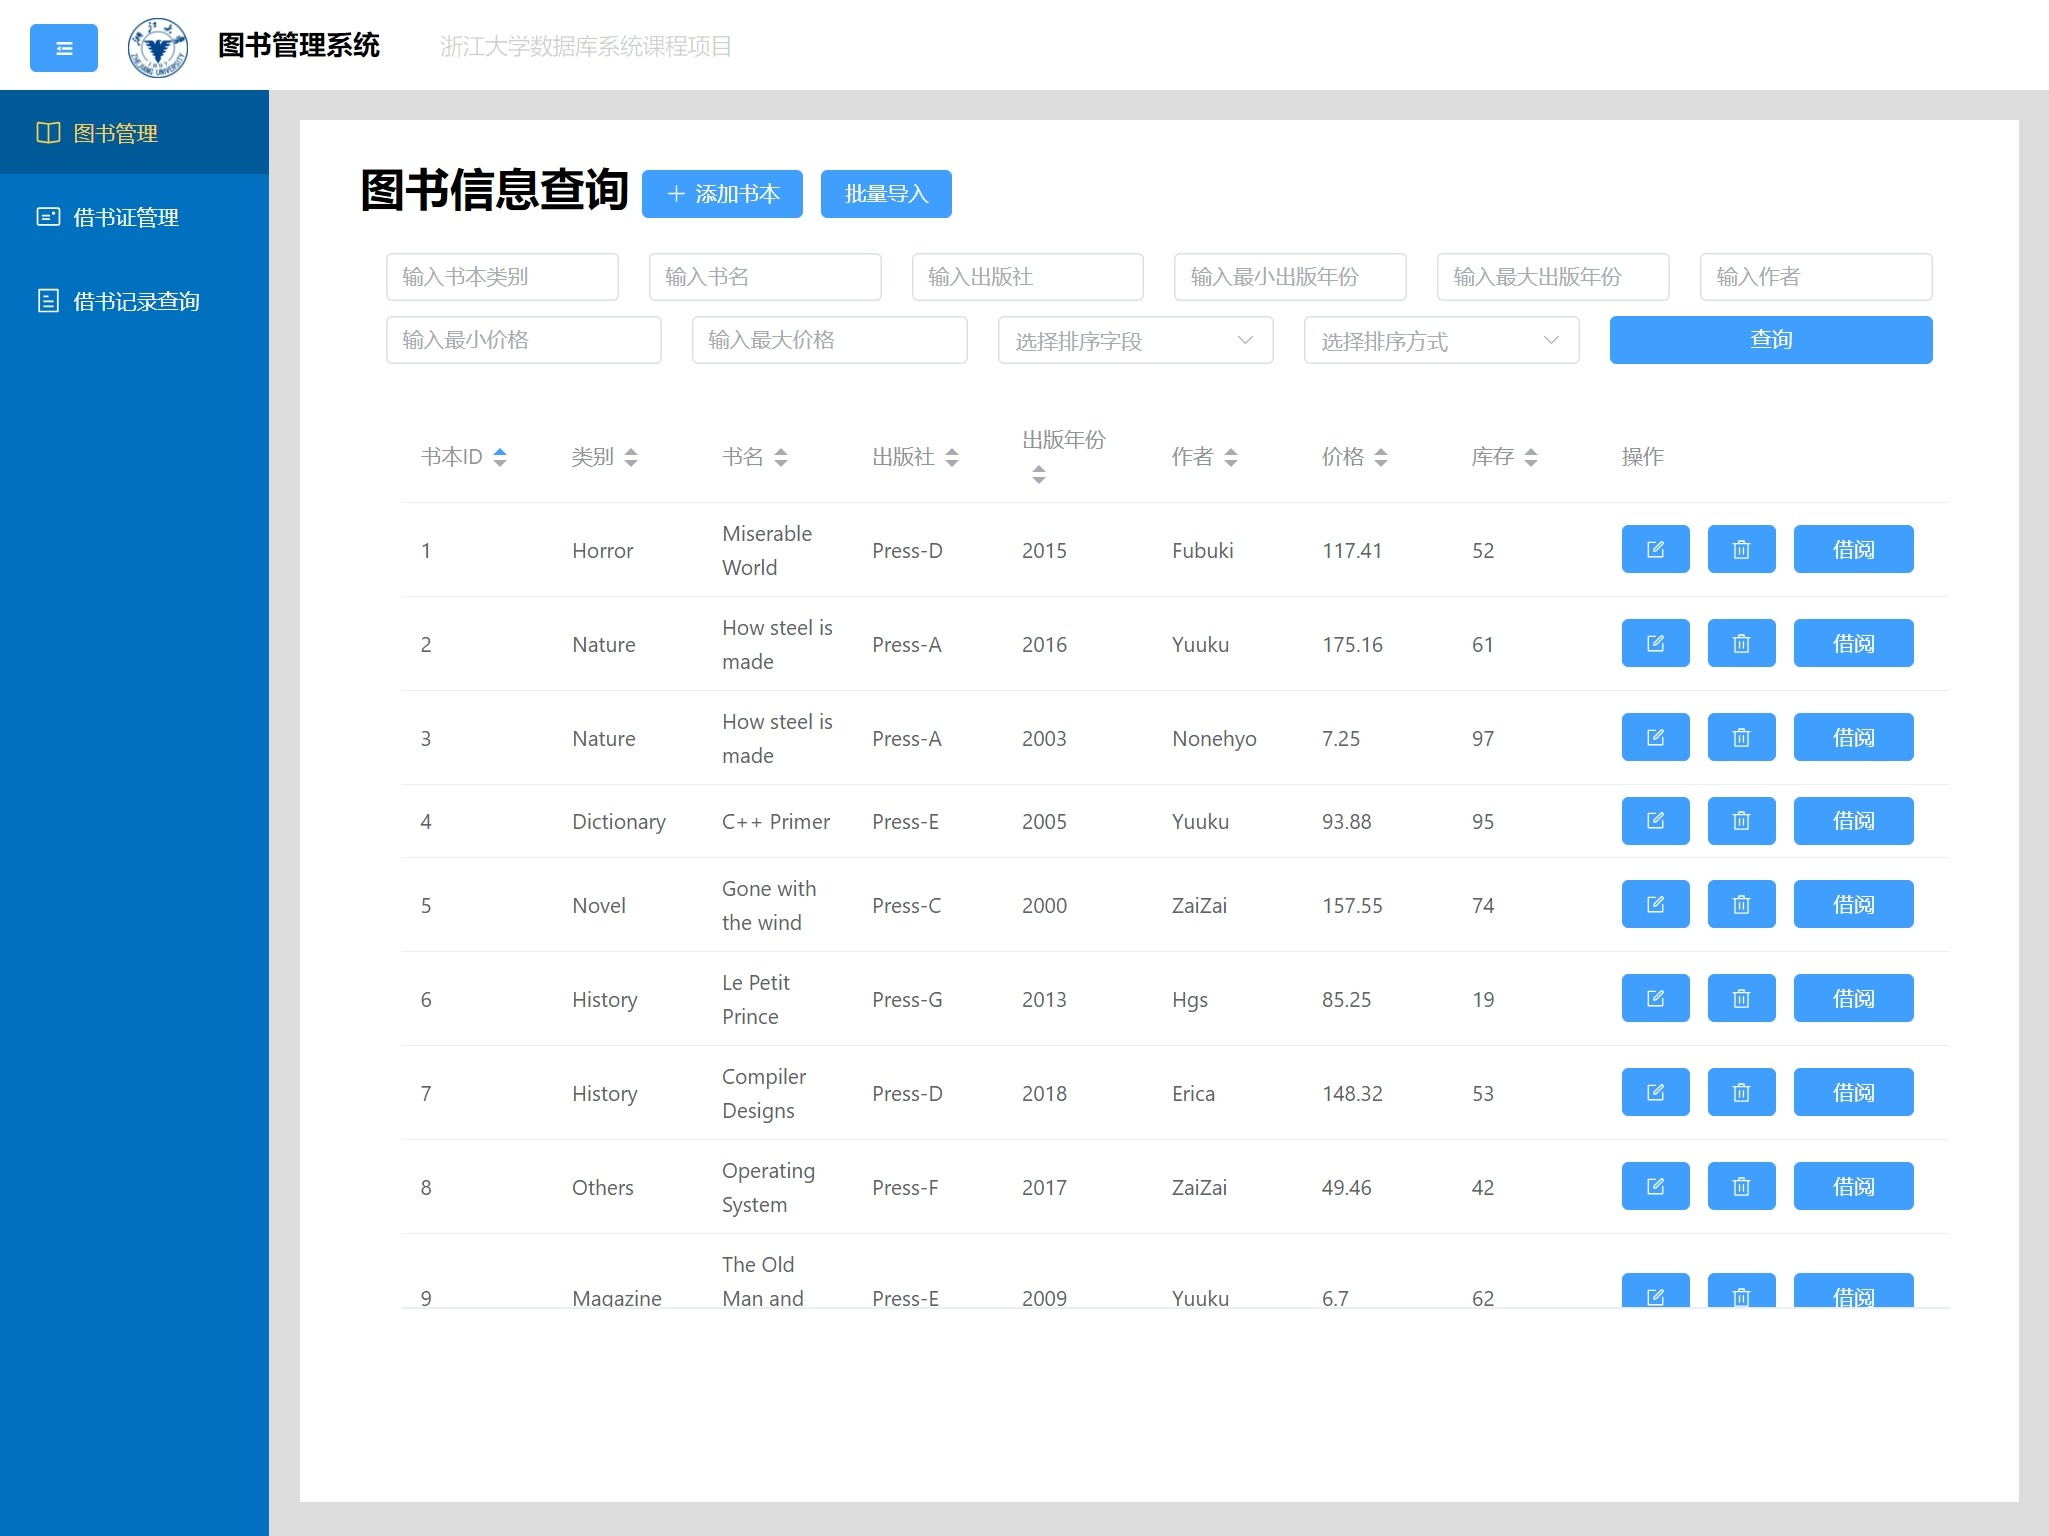
\includegraphics[width=.8\linewidth]{front-book.jpeg}
       \caption{书籍页面}
    \end{subfigure}%
    \begin{subfigure}{.5\linewidth}
       \centering
       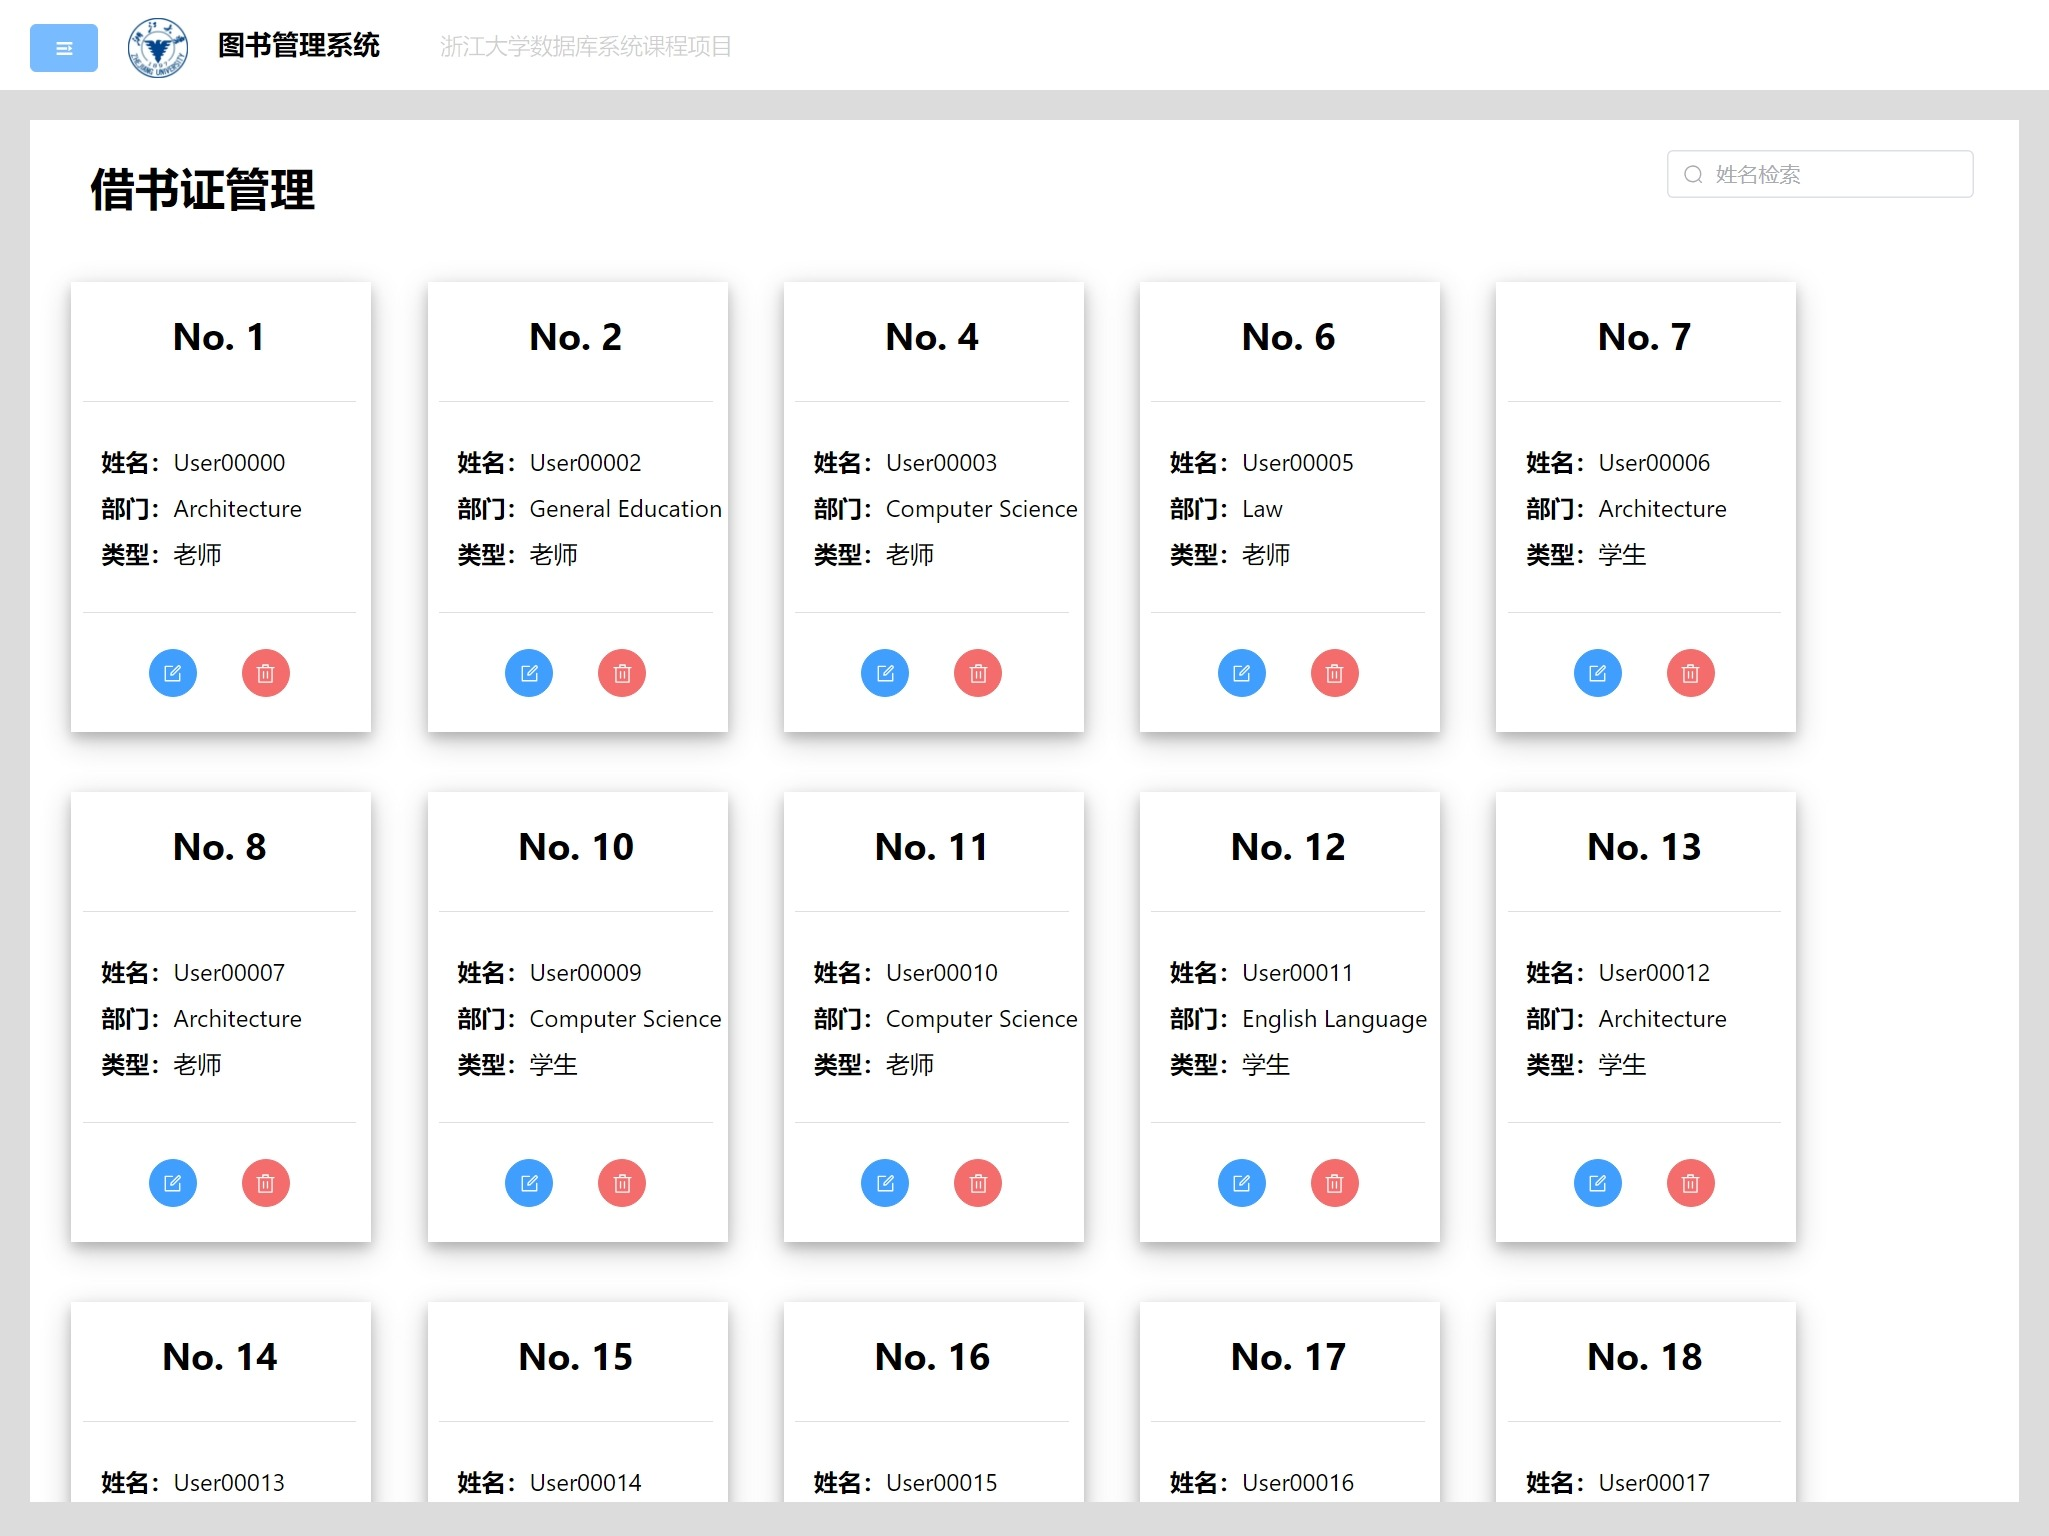
\includegraphics[width=.8\linewidth]{front-card.jpeg}
       \caption{借书卡页面}
    \end{subfigure}
    \begin{subfigure}{.5\linewidth}
       \centering
       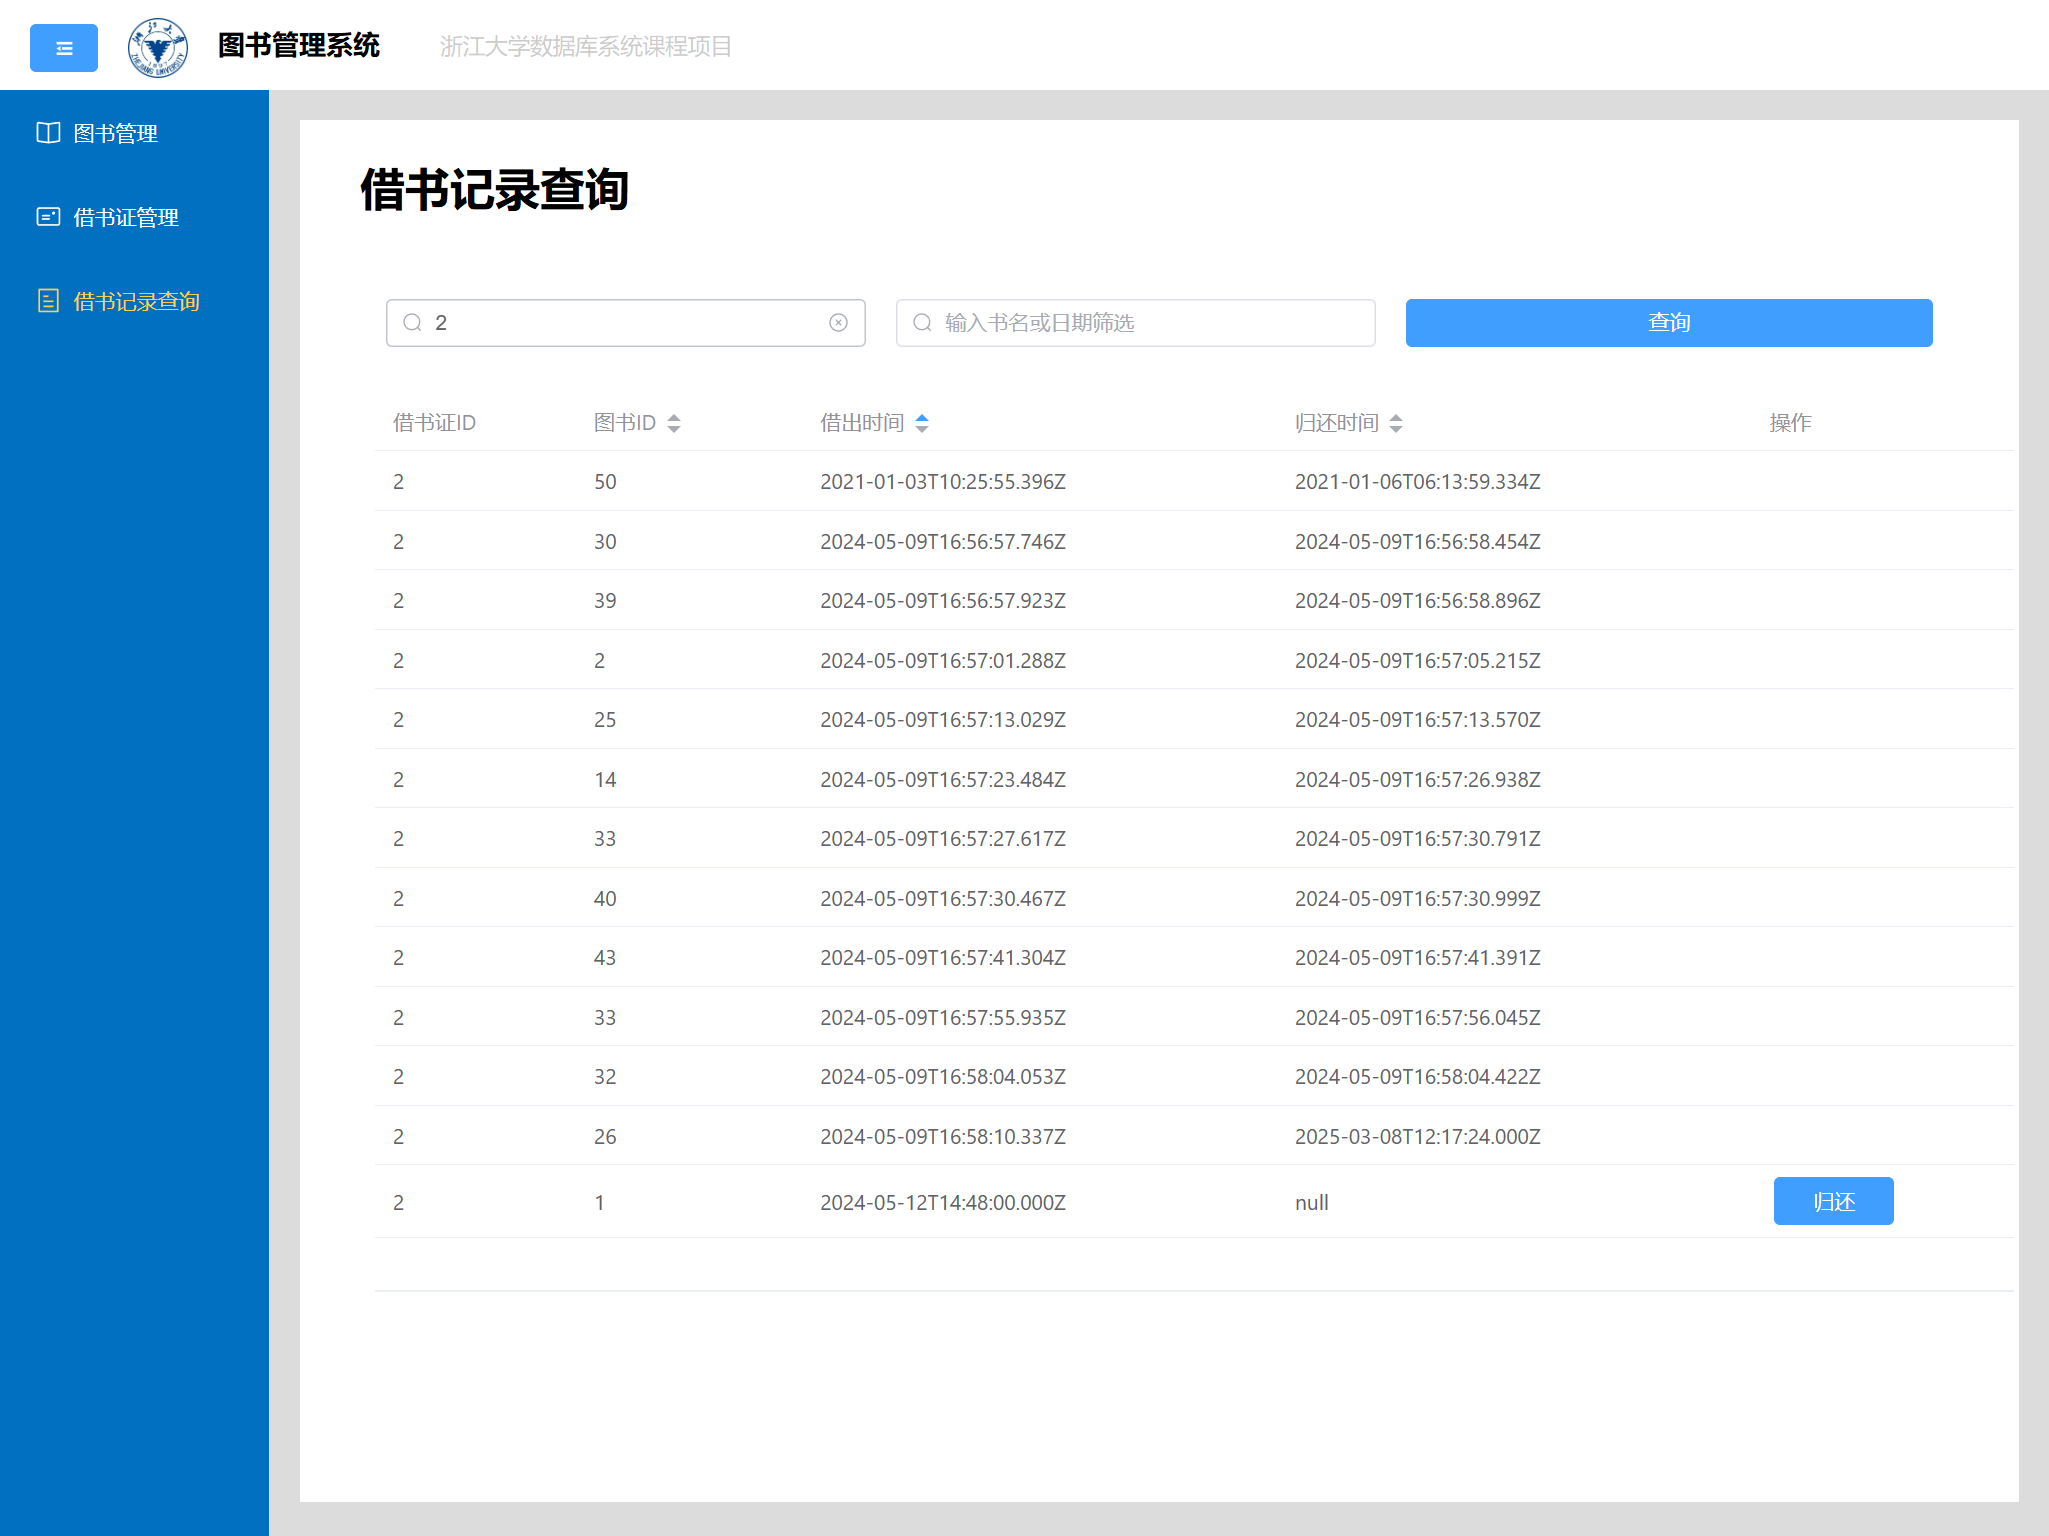
\includegraphics[width=.8\linewidth]{front-borrow}
       \caption{借书记录页面}
    \end{subfigure}
    \caption{前端界面设计}
    \label{fig:front-design}
\end{figure}

我进一步考虑了页面对移动端的兼容性,对整体页面进行了一些改进:

\begin{itemize}
    \item 为侧边栏添加了展开/折叠按钮。
    \item 修改 Header 的溢出表现,改进前“浙江大学数据库系统课程项目”等文字会溢出页首下方,影响侧边栏,改进后溢出部分由 \verb|...| 省略号替代。
    \item 使用 \verb|flex| 对页面上的元素灵活布局。
    \item 使用 \verb|min-width, max-width| 灵活调整对话框的大小,使得桌面端和移动端都能有良好的体验。
\end{itemize}

最终效果如图~\ref{fig:front-phone}~所示。具体实现如代码清单~\ref{lst:fold}~和~\ref{lst:css}~所示。

\begin{figure}[!ht]
    \centering
    \begin{subfigure}{.2\linewidth}
        \centering
        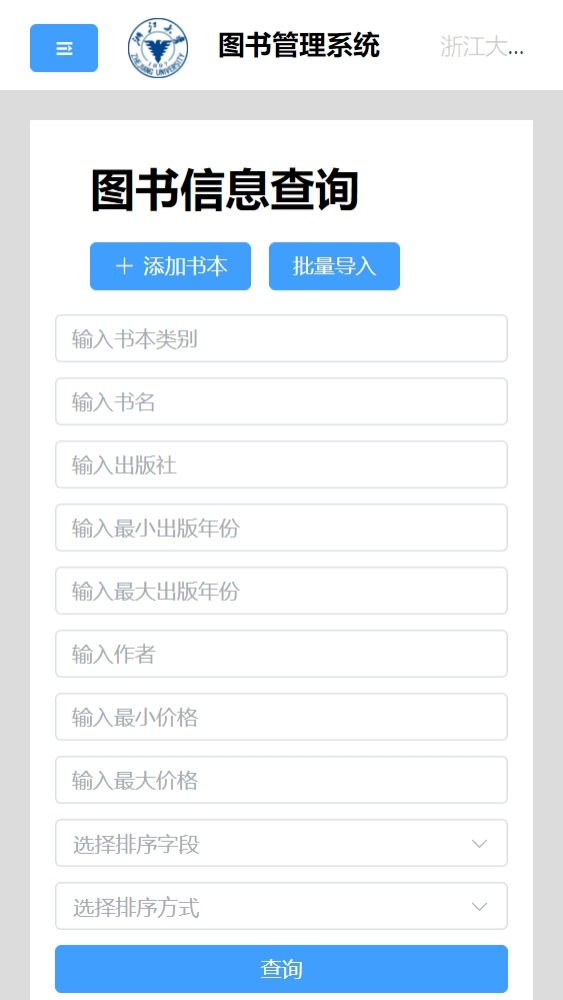
\includegraphics[width=0.8\linewidth]{front-phone.jpeg}
        \caption{移动端界面}
        \label{fig:front-phone}
    \end{subfigure}%
    \begin{subfigure}{.2\linewidth}
        \centering
        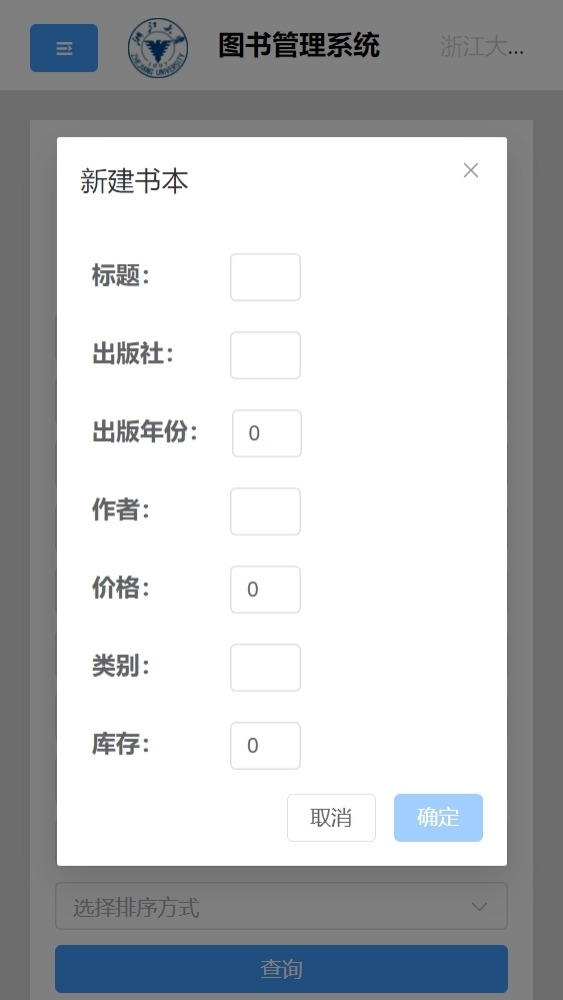
\includegraphics[width=0.8\linewidth]{diag-small.jpeg}
        \caption{移动端对话框(固定)}
        \label{fig:diag-small}
    \end{subfigure}%
    \begin{subfigure}{.5\linewidth}
        \centering
        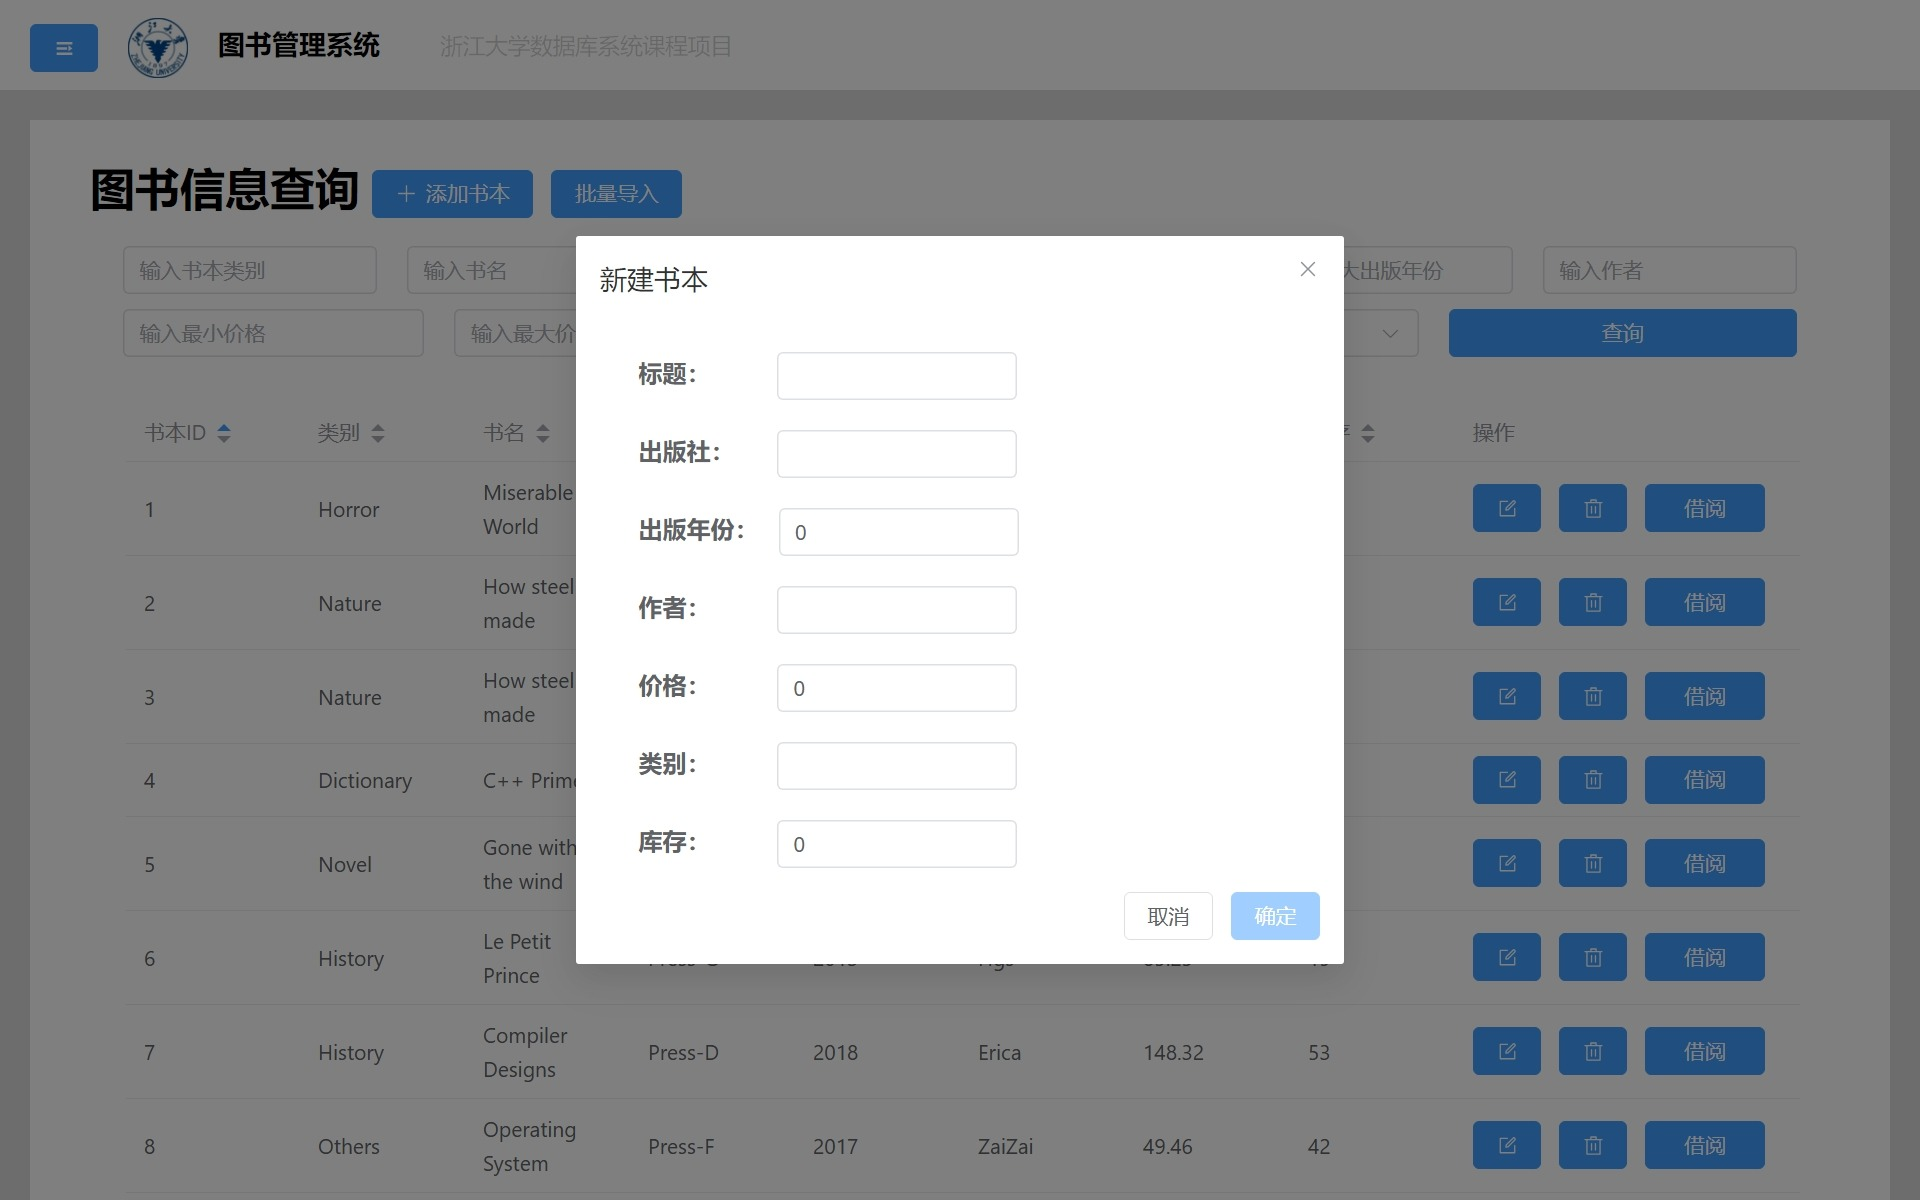
\includegraphics[width=0.9\linewidth]{diag-large.jpeg}
        \caption{桌面端对话框(占比)}
        \label{fig:diag-large}
    \end{subfigure}
    \caption{多端适配}
    \label{fig:compat}
\end{figure}

\begin{lstlisting}[language=HTML, caption=App.vue,label=lst:fold]
<!-- 折叠按钮 -->
<el-header> 
  <el-button
    type="primary"
    :icon="isCollapse ? 'Expand' : 'Fold'"
    style="color: white; margin-right: 20px; vertical-align: middle"
    @click="toggleSidebar"
  ></el-button>
</el-header>
<!-- 折叠属性 -->
<el-container style="width: 100%">
  <el-aside
    :collapse="isCollapse"
    v-bind:style="{ width: isCollapse ? '0%' : '180px' }"
  >
</el-container>
\end{lstlisting}

\begin{lstlisting}[language=HTML, caption=Book.vue,label=lst:css]
<!-- flxe 布局 -->
<div
  style="
    display: flex;
    flex-wrap: wrap;
    gap: 10px 20px;
    align-items: center;
    justify-content: space-between;
    width: 90%;
    margin: 0 auto;
    padding-top: 2vh;
  "
>
<el-input
  v-model="this.toQueryCategory"
  style="flex: 1; min-width: 150px"
  size="big"
  placeholder="输入书本类别"
></el-input>
<!-- 比例和定宽结合 -->
<el-dialog
  v-model="newBookVisible"
  title="新建书本"
  style="min-width: 300px; max-width: 40%;"
  align-center
>
\end{lstlisting}

\section{功能性部分:后端设计思路}

后端采用 RESTful API 设计,参考~\href{https://learn.microsoft.com/en-us/azure/architecture/best-practices/api-design}{Web API design best practices - Azure Architecture Center}~进行设计。资源及其允许的请求如表~\ref{tab:restful}~所示:

\begin{table}[h!]
    \caption{RESTful API 设计}
    \centering
    \label{tab:restful}
    \begin{tabular}{lcccc}
        \toprule
        资源 & GET & POST & PUT & DELETE \\
        \midrule
        \verb|/books| & 查询 & 入库 & & \\
        \verb|/books/{id}| & & & 修改 & 出库 \\
        \verb|/cards| & 查询 & 注册 & & \\
        \verb|/cards/{id}| & & & 修改 & 注销 \\
        \verb|/cards/{id}/borrows| & 查询 & 借书 & & 还书\\
        \bottomrule
    \end{tabular}
\end{table}

约定使用的状态码含义如表~\ref{tab:code}所示:

\begin{table}[h!]
    \caption{RESTful 状态码约定}
    \centering
    \label{tab:code}
    \begin{tabular}{cccccc}
        \toprule
        状态码 & 200 & 204 & 404 & 405 & 500\\
        \midrule
        含义 & 动作完成 & 用于 \verb|OPTION| 预检 & 资源不存在 & 不允许的操作 & SQL 服务器错误\\
        \bottomrule
    \end{tabular}
\end{table}

接下来是 Java 部分的实现。对于每一个请求,使用 \verb|uri.getPath.split("/")| 分割路径,结合 \verb|Switch| 语句对请求类型进行分类路由,如代码清单~\ref{lst:route}~所示:

\begin{lstlisting}[language=java, caption=路由,label=lst:route]
public void handle(HttpExchange exchange) throws IOException {
    String requestMethod = exchange.getRequestMethod();
    URI uri = exchange.getRequestURI();
    String path = uri.getPath();
    log.log(Level.INFO, "[Web] Request: " + path + " " + requestMethod);
    String[] pathParts = path.split("/");
    switch (pathParts.length) {
        case 2: // /books
        //... 
        case 3: // /books/{bookId}
            try {
                Integer.parseInt(pathParts[2]);
            } catch (NumberFormatException e) {
                exchange.sendResponseHeaders(404, -1);
                return;
            }
            switch (requestMethod) {
                case "PUT":
                    booksIdPut(exchange, pathParts);
                    break;
                case "DELETE":
                    booksIdDelete(exchange, pathParts);
                    break;
                case "OPTIONS":// preflight response
                    exchange.getResponseHeaders().set("Access-Control-Allow-Methods", "PUT, DELETE");
                    exchange.sendResponseHeaders(204, -1);
                    break;
                default:
                    exchange.sendResponseHeaders(405, -1);
                    break;
            }
        default:
            exchange.sendResponseHeaders(404, -1);
            break;
    }
}
\end{lstlisting}

请求的解析涉及消息体或 URL 参数,使用 Java 的库都能轻松解决,如代码清单~\ref{lst:parse}~所示:

\begin{lstlisting}[language=java, caption=请求解析,label=lst:parse]
// URL 参数
private static Map<String, String> parseQueryParams(String query) {
    Map<String, String> queryParams = new HashMap<>();
    String[] params = query.split("&")
    for (String param : params) {
        String[] keyValue = param.split("=");
        String key = keyValue[0];
        String value = keyValue.length > 1 ? keyValue[1] : null;
        queryParams.put(key, value);
    return queryParams;
}
private void booksGet(HttpExchange exchange) throws IOException {
    String s = exchange.getRequestURI().getQuery();
    Map<String, String> queryParams = parseQueryParams(s)
    String category = getQueryParam(queryParams, "category");
    //...
}
// JSON 消息体
public Card(JSONObject json) {
    this.cardId = json.getInteger("cardId") == null ? 0 : json.getInteger("cardId");
    this.name = json.getString("name");
    this.department = json.getString("department");
    this.type = CardType.values(json.getString("type"));
}
private void cardsIdPut(HttpExchange exchange, String[] pathParts) throws IOException {
    String requestBody = new BufferedReader(new InputStreamReader(exchange.getRequestBody())).lines().collect(Collectors.joining("\n"));
    Card card = new Card(JSONObject.parseObject(requestBody));
    ApiResult ar = library.modifyCardInfo(card)
    makeResponse(exchange, ar);
}
\end{lstlisting}

HTTP 消息体中携带的信息可以是 JSON 或者错误信息,如代码清单~\ref{lst:httpbody}~展示了一个包装函数 \verb|makeResponse()| 用于根据 MySQL 服务器的返回生成简单的 HTTP 响应。

\begin{lstlisting}[language=java, caption=消息体,label=lst:httpbody]
// 简单响应
private static void makeResponse(HttpExchange exchange, ApiResult ar) throws IOException {
    exchange.sendResponseHeaders(ar.ok ? 200 : 500, 0);
    if (!ar.ok) {
        exchange.getResponseHeaders().set("Content-Type", "text/plain");
        OutputStream outputStream = exchange.getResponseBody();
        outputStream.write(ar.message.getBytes());
        outputStream.close();
    }
}
// JSON 消息体
private void cardsGet(HttpExchange exchange) throws IOException {
    ApiResult ar = library.showCards()
    CardList cardList = (CardList) ar.payload;
    JSONArray jsonArray = new JSONArray();
    List<Card> lc = cardList.getCards();
    for (Card c : lc) {
        jsonArray.add(JSONObject.parseObject(c.toJson()));
    exchange.getResponseHeaders().set("Content-Type", "application/json");
    exchange.sendResponseHeaders(200, 0);
    OutputStream outputStream = exchange.getResponseBody();
    outputStream.write(jsonArray.toJSONString().getBytes());
    outputStream.close();
}
\end{lstlisting}

对应地,在 Axios 中,将根据消息状态码和消息体进行处理。代码清单~\ref{lst:axios}~展示了 Axios 中通用的 HTTP 消息处理模式。值得一提的是,Axios 认为非 \verb|2XX| 的状态码均表示错误,使用 \verb|catch| 才能处理。

\begin{lstlisting}[language=javascript, caption=Axios,label=lst:axios]
methods: {
  async ConfirmRemoveBook() {
    axios
      .delete(`/books/${this.toRemove}`)
      .then(() => {
        this.Success();
        this.removeBookVisible = false;
        this.QueryBooks();
      })
      .catch((error) => {
        this.ErrorHandling(error);
      });
  },
  Success() {
    ElMessage.success("操作成功");
  },
  ErrorHandling(error) {
    if (error.response) {
      ElMessage.error("操作失败:" + error.response.data);
      console.log(error.response.data);
      console.log(error.response.status);
      console.log(error.response.headers);
    } else if (error.request) {
      ElMessage.error("服务器无返回:" + error.request);
      console.log(error.request);
    } else {
      ElMessage.error("网页内部错误:" + error.message);
      console.log("Error", error.message);
    }
  },
}
\end{lstlisting}

\section{部署}

修改 \verb|pom.xml| 的 \verb|<build>| 部分,生成 \verb|.jar| 文件。

\begin{lstlisting}[language=xml, caption=pom.xml,label=lst:pom]
<packaging>jar</packaging>
<build>
    <resources>
        <resource>
            <directory>src/main/resources</directory>
            <filtering>false</filtering>
        </resource>
    </resources>
    <plugins>
        <plugin>
            <groupId>org.apache.maven.plugins</groupId>
            <artifactId>maven-jar-plugin</artifactId>
            <version>3.4.1</version>
        </plugin>
        <plugin>
            <groupId>org.apache.maven.plugins</groupId>
            <artifactId>maven-shade-plugin</artifactId>
            <version>3.2.4</version>
            <executions>
                <execution>
                    <phase>package</phase>
                    <goals>
                        <goal>shade</goal>
                    </goals>
                    <configuration>
                        <minimizeJar>true</minimizeJar>
                        <filters>
                            <filter>
                                <artifact>*:*</artifact>
                                <excludes>
                                    <exclude>META-INF/*.SF</exclude>
                                    <exclude>META-INF/*.DSA</exclude>
                                    <exclude>META-INF/*.RSA</exclude>
                                </excludes>
                            </filter>
                        </filters>
                        <artifactSet>
                            <excludes>
                                <exclude>junit:junit</exclude>
                                <exclude>jmock:*</exclude>
                                <exclude>*:xml-apis</exclude>
                                <exclude>org.apache.maven:lib:tests</exclude>
                                <exclude>log4j:log4j:jar:</exclude>
                            </excludes>
                        </artifactSet>
                    </configuration>
                </execution>
            </executions>
        </plugin>
    </plugins>
</build>
\end{lstlisting}

当 \verb|resource| 打包进入 \verb|.jar| 后,不可再视为文件,只能使用流读取,因此 \verb|ConnectConfig()| 也需要做相应修改:

\begin{lstlisting}[language=java, caption=更改为流读取,label=lst:stream]
public ConnectConfig() throws FileNotFoundException {
    InputStream stream = ConnectConfig.class.getClassLoader().getResourceAsStream("application.yaml");
    if (stream == null) {
        throw new FileNotFoundException();
    }
    InputStreamReader isr = new InputStreamReader(stream);
    Yaml yaml = new Yaml();
    Map<String, Object> objectMap = yaml.load(isr);
    //...
}
\end{lstlisting}

修改前端 \verb|package.json| 使其监听目标为宿主机的请求。修改 \verb|main.js|,将 Axios 请求定向到后端主机名 \verb|https://|。

\begin{lstlisting}[caption=前端配置,label=lst:front]
// package.json
"scripts": {
  "dev": "vite --host",
  "build": "vite build",
  "preview": "vite preview"
},
// main.js
axios.defaults.baseURL = 'https://';
\end{lstlisting}

为站点创建 Nginx 配置文件进行反向代理,以后端为例,配置文件如代码清单~\ref{lst:nginx}~所示。我选择将一部分 CORS 控制头(如 \verb|Access-Control-Allow-Origin|)交给反代服务器,因为这些头和站点本身强相关,应当由反代服务器而不是后端进行处理。

\begin{lstlisting}[caption=Nginx 反代,label=lst:nginx]
server {
    error_log /var/log/nginx/lab5-api.log;
    server_name  ;

    location / {
        add_header 'Access-Control-Allow-Origin' '' always;
        add_header 'Access-Control-Allow-Credentials' 'true' always;
        add_header 'Access-Control-Allow-Headers' '*' always;
        add_header 'Access-Control-Max-Age' '86400' always;
        #add_header 'Vary' "Accept-Encoding, Origin";
        proxy_pass http://127.0.0.1:8000;
        proxy_set_header Host $proxy_host;
        proxy_set_header X-Real-IP $remote_addr;
        proxy_set_header X-Forwarded-For $proxy_add_x_forwarded_for;
    }

    listen 443 ssl; # managed by Certbot
    ssl_certificate /etc/letsencrypt/live//fullchain.pem; # managed by Certbot
    ssl_certificate_key /etc/letsencrypt/live//privkey.pem; # managed by Certbot
    include /etc/letsencrypt/options-ssl-nginx.conf; # managed by Certbot
    ssl_dhparam /etc/letsencrypt/ssl-dhparams.pem; # managed by Certbot
}
server {
    if ($host = ) {
        return 301 https://$host$request_uri;
    } # managed by Certbot

    listen       80;
    server_name  ;
    return 404; # managed by Certbot
}
\end{lstlisting}

在服务器上运行前后端:

\begin{lstlisting}[language=xml, caption=pom.xml,label=lst:pom]
java -cp ./LibraryManagementSystem-FINAL.jar Main
npm run dev
\end{lstlisting}

后端主程序和数据库部分均使用 \verb|java.util.logging| 进行日志记录,能够清晰地了解后端对响应的处理情况。

\begin{lstlisting}[caption=日志,label=lst:log]
root@iZbp1ah8iba4f0no3ydfe0Z ~/db-lab5# java -cp ./LibraryManagementSystem-FINAL.jar Main
ZJUDB LibMgmt Backend Version Final.
Editor: bowling
INFO: [DB] Success to connect database. [Sun May 12 20:30:22 CST 2024]
May 12, 2024 8:30:22 PM LibraryManagementSystemImpl <init>
INFO: LibraryManagementSystemImpl created
INFO: [Web] Server started on port 8000. [Sun May 12 20:30:22 CST 2024]
INFO: [Web] Request: /books GET [Sun May 12 20:54:01 CST 2024]
INFO: [Web] /books: GET. [Sun May 12 20:54:01 CST 2024]
INFO: [DB] Query for book 
BookQueryConditions {category='null', title='null', press='null', minPublishYear=null, maxPublishYear=null, author='null', minPrice=null, maxPrice=null, sortBy=BOOK_ID, sortOrder=ASC} [Sun May 12 20:54:01 CST 2024]
INFO: [Web] Request: /cards/0/borrows OPTIONS [Sun May 12 20:54:06 CST 2024]
INFO: [Web] Request: /cards/0/borrows POST [Sun May 12 20:54:06 CST 2024]
INFO: [Web] /cards/{id}/borrows: POST. [Sun May 12 20:54:06 CST 2024]
May 12, 2024 8:54:06 PM LibraryManagementSystemImpl borrowBook
SEVERE: Cannot add or update a child row: a foreign key constraint fails (`library`.`borrow`, CONSTRAINT `borrow_ibfk_1` FOREIGN KEY (`card_id`) REFERENCES `card` (`card_id`) ON DELETE CASCADE ON UPDATE CASCADE)
java.sql.SQLIntegrityConstraintViolationException: Cannot add or update a child row: a foreign key constraint fails (`library`.`borrow`, CONSTRAINT 
`borrow_ibfk_1` FOREIGN KEY (`card_id`) REFERENCES `card` (`card_id`) ON DELETE CASCADE ON UPDATE CASCADE)
        at com.mysql.cj.jdbc.exceptions.SQLError.createSQLException(SQLError.java:117)
...
\end{lstlisting}

\chapter{问题与解决方法}

\section{本地 MySQL 并行测试通过,但远程 MySQL 服务器并行测试无法通过}

这段代码显然不满足一致性的要求,借书和库存的变化没有作为一个整体。在本地测试时网络延迟低,两个事务能够快速被处理。经过多次测试,使用的 16 个线程都侥幸没有触发错误。但使用远程 MySQL 服务器时,其中就有 3-4 个线程开始出现错误。从这里我们可以看到测试环境和生产环境的不同,这是我们进行测试时需要保持关注的。

决方法是将所有操作合并到一起,在最后进行 \verb|commit()|。这样在事务隔离为串行级别时能够处理并发请求。在考虑性能和具体应用的场景下,应当使用锁。

\begin{lstlisting}[language=java, caption=Q1,label=lst:q1]
public ApiResult borrowBook(Borrow borrow) {
    Connection conn = connector.getConn();
    // set serializable isolation level
    try {
        conn.setTransactionIsolation(Connection.TRANSACTION_SERIALIZABLE);
        // if user has borrowed the book, return error
        PreparedStatement stmt = conn.prepareStatement("SELECT * FROM borrow WHERE card_id = ? AND book_id = ? AND return_time = 0");
        stmt.setInt(1, borrow.getCardId());
        stmt.setInt(2, borrow.getBookId());
        ResultSet rs = stmt.executeQuery();
        if (rs.next()) {
            return new ApiResult(false, "Book already borrowed");
        }
    } catch (Exception e) {
        rollback(conn);
        LOGGER.log(Level.SEVERE, e.getMessage());
        e.printStackTrace();
        return new ApiResult(false, e.getMessage());
    }
    try{
        // if book is out of stock, return error
        PreparedStatement stmt = conn.prepareStatement("SELECT stock FROM book WHERE book_id = ?");
        stmt.setInt(1, borrow.getBookId());
        ResultSet rs = stmt.executeQuery();
        if (!rs.next()) {
            return new ApiResult(false, "Book not found");
        }
        int stock = rs.getInt("stock");
        if (stock == 0) {
            return new ApiResult(false, "Book out of stock");
        }
    } catch (Exception e) {
        rollback(conn);
        LOGGER.log(Level.SEVERE, e.getMessage());
        e.printStackTrace();
        return new ApiResult(false, e.getMessage());
    }
    try{
        // borrow book
        PreparedStatement stmt = conn.prepareStatement("INSERT INTO borrow (card_id, book_id, borrow_time) VALUES (?, ?, ?)");
        stmt.setInt(1, borrow.getCardId());
        stmt.setInt(2, borrow.getBookId());
        stmt.setLong(3, borrow.getBorrowTime());
        stmt.executeUpdate();
        commit(conn);
    } catch (Exception e) {
        rollback(conn);
        LOGGER.log(Level.SEVERE, e.getMessage());
        e.printStackTrace();
        return new ApiResult(false, e.getMessage());
    }
    try{
        // decrease stock
        PreparedStatement stmt = conn.prepareStatement("UPDATE book SET stock = stock - 1 WHERE book_id = ?");
        stmt.setInt(1, borrow.getBookId());
        stmt.executeUpdate();
        commit(conn);
    } catch (Exception e) {
        rollback(conn);
        LOGGER.log(Level.SEVERE, e.getMessage());
        e.printStackTrace();
        return new ApiResult(false, e.getMessage());
    }
    return new ApiResult(true, null);
}
\end{lstlisting}

\section{构建和运行 jar 文件}

因为计划部署到服务器上,所以需要构建一个 \verb|.jar| 文件。当然,能直接构建 Docker 更好,但查到的资料不是很多。

由于是第一次构建 Java 项目,对 Maven 也不熟,浪费了不少时间在上面,尝试了很多插件和依赖处理办法等。遇到过的错误有:

\begin{itemize}
    \item 各种编译和依赖问题:\verb|Invalid signature file digest for Manifest main attributes...|。
    \item Maven test 出现问题 \verb|The forked VM terminated without properly saying googbye. VM crash ...|,只能跳过。
    \item \verb|.jar| 文件中只有 \verb|Main|,没有其他依赖。
    \item 在前文提及的 \verb|resource| 放置在 \verb|.jar| 文件中如何读取的问题。
    \item \verb|java -jar| 找不到 \verb|MANIFEST| 或找不到其中的类 \verb|Error: Could not find or load main class Main while executing jar file.|。
\end{itemize}

最后的解决办法是使用 \verb|maven-shade-plugin| 插件对依赖进行处理、删除某些签名的 \verb|jar| 文件的签名,具体的配置已在前文展示。运行时,使用 \verb|java -cp| 指定 ClassPath。

希望实验手册能够对 Maven 的构建过程特别是 \verb|.jar| 文件的生成给出一些必要的提示。

\section{前端无法收到 2XX 以外消息的消息体}

在约定中,500 表示 SQL 服务器产生了错误信息,错误信息应当以文本的形式作为消息体传递给前端并展示。但是测试时,Axios 的 \verb|error.response| 是空的,表现为 Network Error,这非常奇怪。

使用浏览器开发者工具,控制台显示 CORS 被拒,浏览器也确实没有接受消息体。可是我已经在 Nginx 中配置好了 CORS,怎么回事呢?

很可惜配置了 HTTPS 所以 WireShark 无法抓包。因为不是很信任浏览器说的话,我又使用 Postman 构造请求,结果响应头中确实没有 CORS。从而断定是 Nginx 的问题。

查阅资料得知:Unfortunately \verb|add_header| won't work with status codes other than 200, 204, 301, 302 or 304. 在 Nginx 为响应的选项添加 \verb|always| 即可解决改问题。

\section{Axios 是如何看待状态码的?}

起初我试图在 \verb|.then()| 中使用 \verb|response.status| 进行判断,为 500 错误码设置弹窗。但是,怎么都弹不出来。打印到控制台,发现根本没进 \verb|.then()|。

Axios 如何 Handle 非 2XX 状态码这个问题在 GitHub 上有不少讨论,有人使用 \verb|config| 修改 \verb|validateStatus|,因为 Axios 基于它判定异常处理,不过被认为是 Hack 而不建议泛用。所以我也选择了使用异常处理。\cite{Ijaz}

不过这也让我思考在 RESTful API 中状态码的意义。它究竟应该代表对对象操作的执行情况,还是用于表示网络通信情况呢?如果我收到了 500 的回复,是网络通信、基础设施故障的问题还是对对象的操作没有成功?

此外,使用 Axios 发送 DELETE 请求时,携带请求体的格式也与其他请求不一样,需要注意。\cite{Axios}

\section{在服务器上运行一段时间后,后端响应全部失败}

部署在服务器上,一段时间后访问发现后端返回值为空。登录服务器查询日志:

\begin{lstlisting}[caption=日志,label=lst:log-long]
Caused by: com.mysql.cj.exceptions.CJCommunicationsException: The last packet successfully received from the server was 38,363,785 milliseconds ago. The last packet sent successfully to the server was 38,363,787 milliseconds ago. is longer than the server configured value of 'wait_timeout'. You should consider either expiring and/or testing connection validity before use in your application, increasing the server configured values for client timeouts, or using the Connector/J connection property 'autoReconnect=true' to avoid this problem.
\end{lstlisting}

在设计时,我出于性能(和服务器资源)的考虑,选择让程序启动时就与 MySQL 服务器建立连接,之后持续复用连接。我看到身边有同学选择在每次收到请求时建立连接,感觉这种做法的适用性比较局限。然而 MySQL 是有超时限制的,因此需要修改 \verb|DatabaseType.java| 中的 \verb|url| 方法,添加 \verb|?autoReconnect=true| 即可。

\section{时间戳问题}

查看源码可以发现,单元测试中在数据库存储的时间是 UNIX 时间戳,将其直接展示到前端是非常不友好的。考虑在后端 \verb|toJson| 函数将其转换为 ISO 8601 表示如 \verb|yyyy-mm-dd hh:mm:ss|。让 Copilot 写了一通,看起来不错。用户在前端进行输入时,转换为 UNIX 时间戳发回后端查询,也挺好。

结果在还书测试时失败了:Book Not Borrowed。这条借书记录明明就在表上,怎么会查不到呢?

所幸调试前端时在控制台打印了转换的时间戳,发现后三位始终为 0。原来毫秒级别的 UNIX 时间戳转换为 ISO 8601 应当完整地表示为如 \verb|2024-05-12T14:48:06.331Z| 的格式,这一信息从后端发出时就已丢失,当然无法找到对应的借书记录。Copilot 再背一锅。

最后选择在前后端之间传递时间戳,由前端统一处理 UNIX 时间戳与 ISO 8601 的转换。

\section{注入攻击}

做 Lab 的同学应该都能意识到 SQL 注入的危害,并使用参数化查询进行规避。但是,对于课外的 JSON 可能就会忽略。我就犯了这样的错误,被同学发现了:

\begin{figure}[!h]
    \centering
    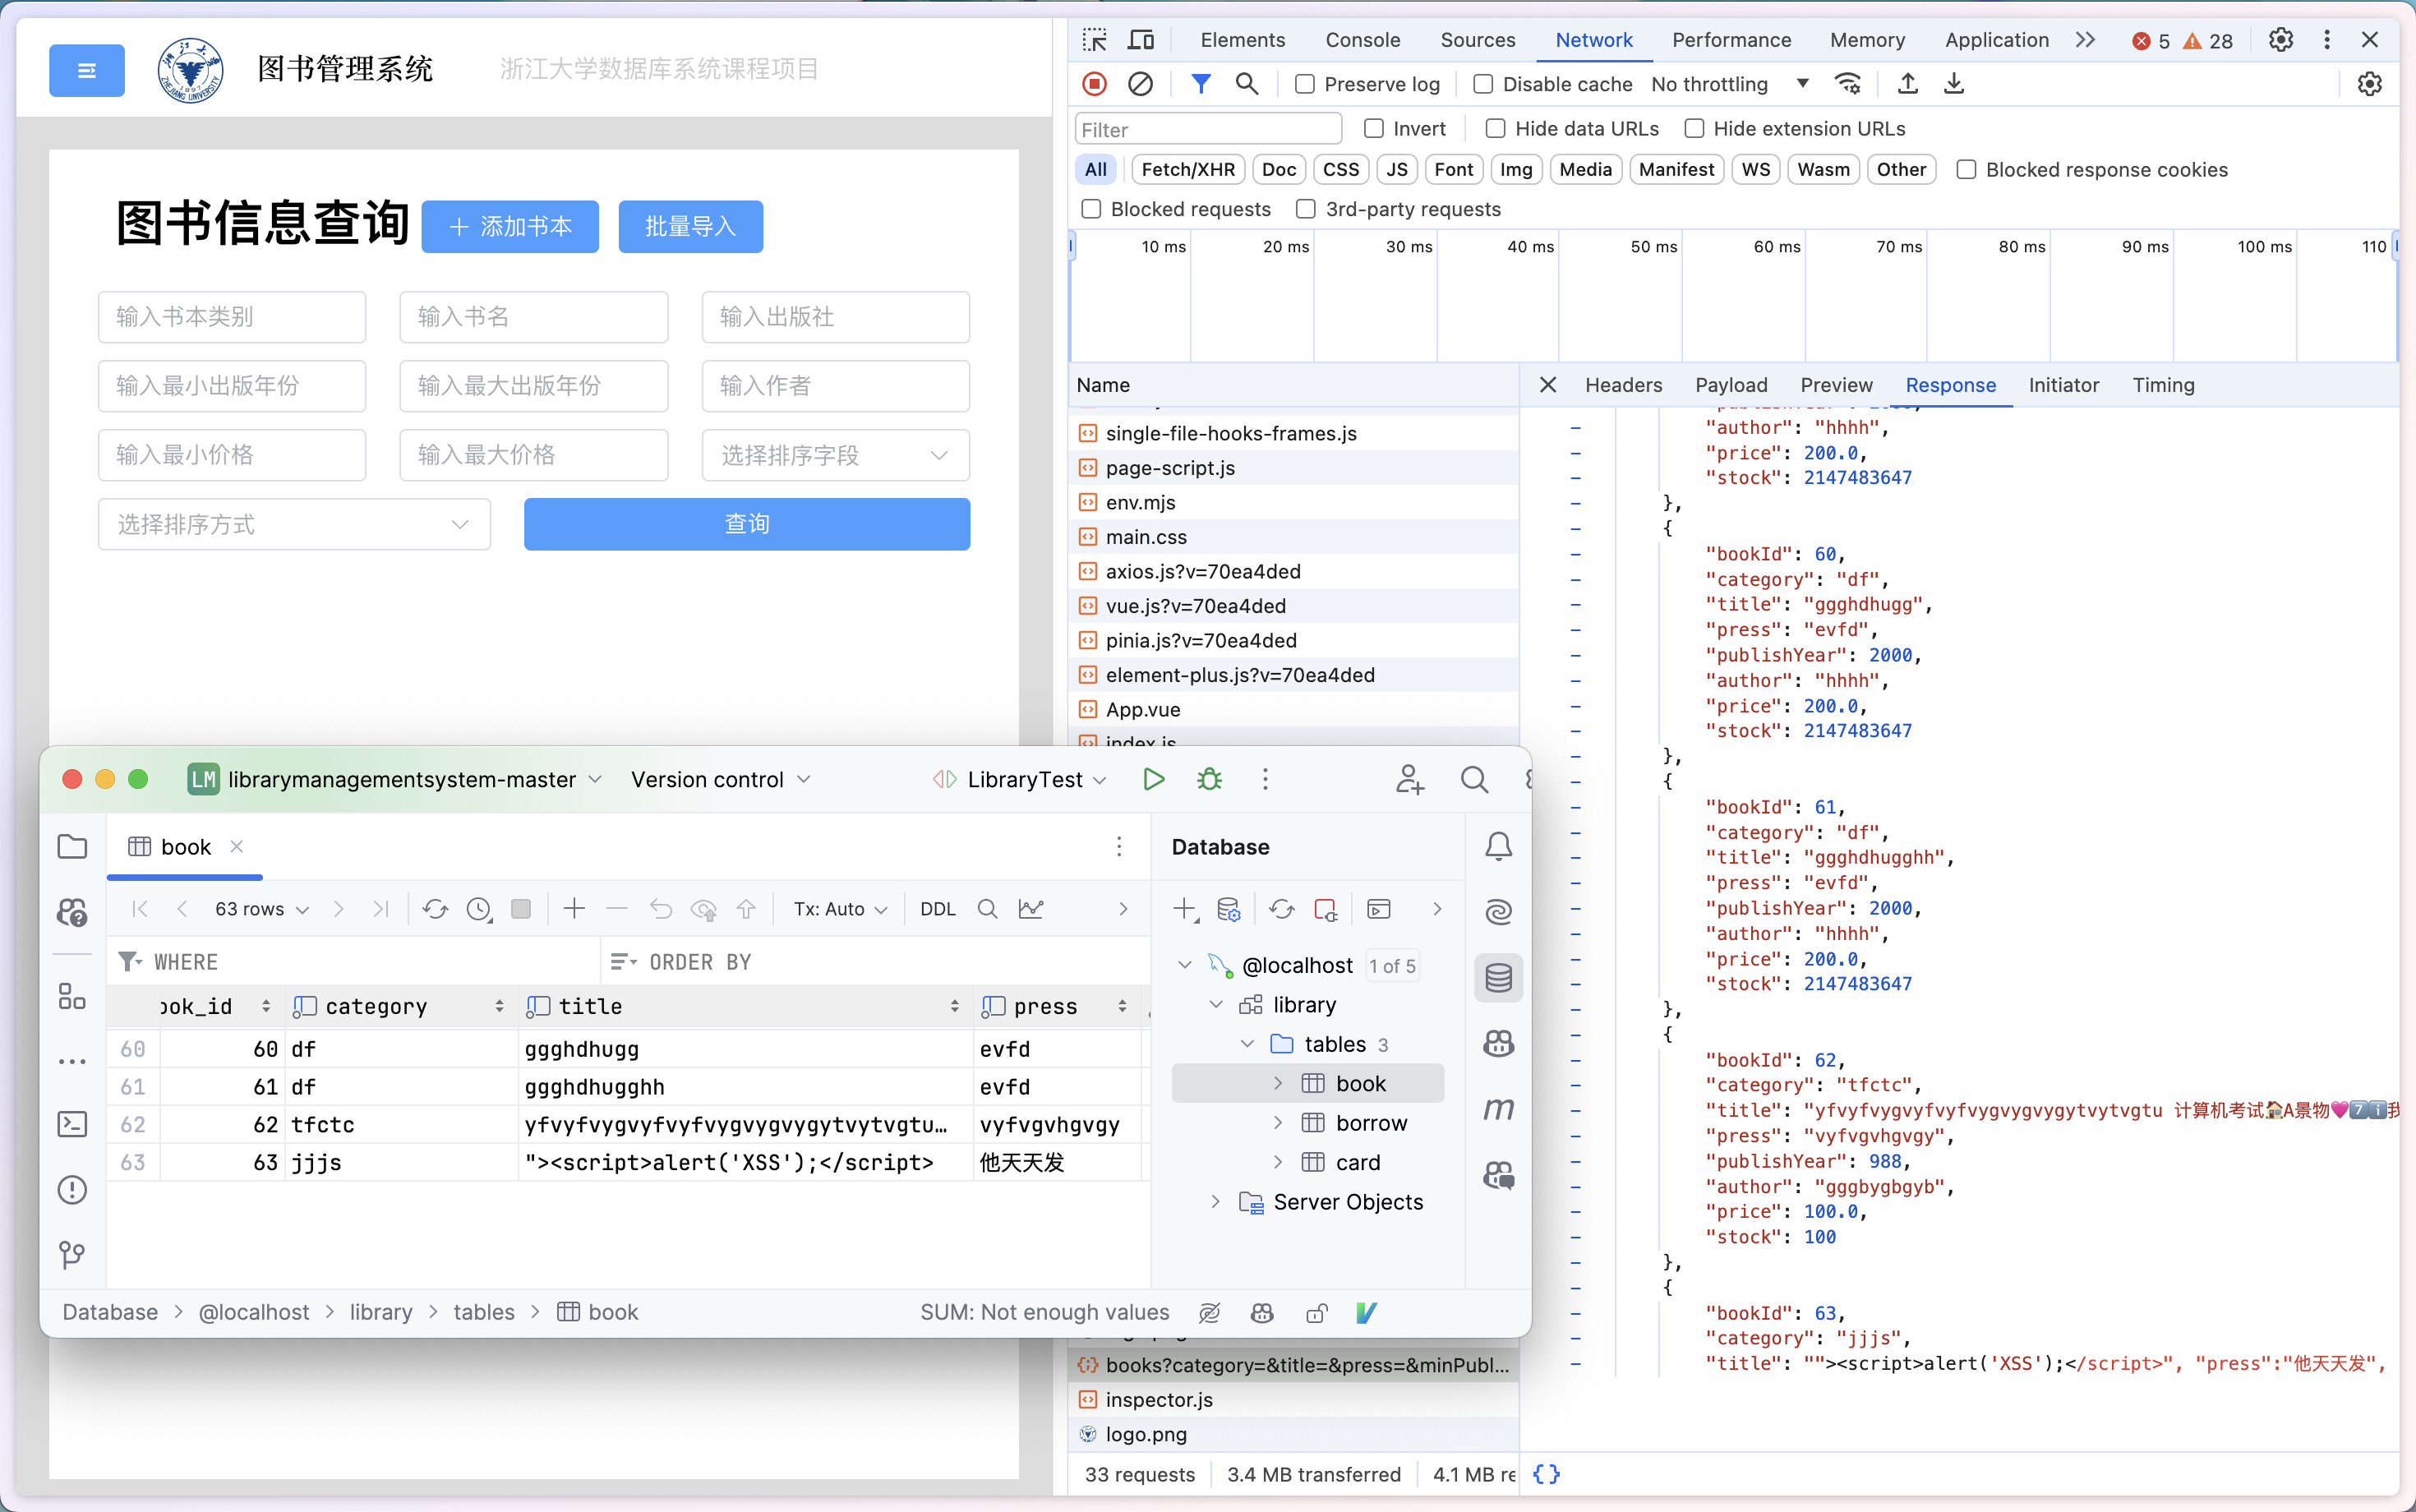
\includegraphics[width=\textwidth]{src/attack-json.png}
    \caption{JSON“注入攻击”}
    \label{fig:json-attack}
\end{figure}

同学发起了书名为 \verb|"><script>alert('XSS');</script>| 的提交,成功进入数据库。但是我从数据库返回的结果构建 JSON 使用的是字符串拼接,从上图可以看到消息体中的 JSON 完全乱套了,Vue 在控制台中提示数据错误如~\ref{fig:vue}~所示,图书页面的表格无法显示。将构建 JSON 的方法改为 \verb|JSONObject.put()| 即可解决问题,正常显示。

\begin{figure}[!h]
\centering
    \begin{subfigure}{0.5\linewidth}
    \centering
    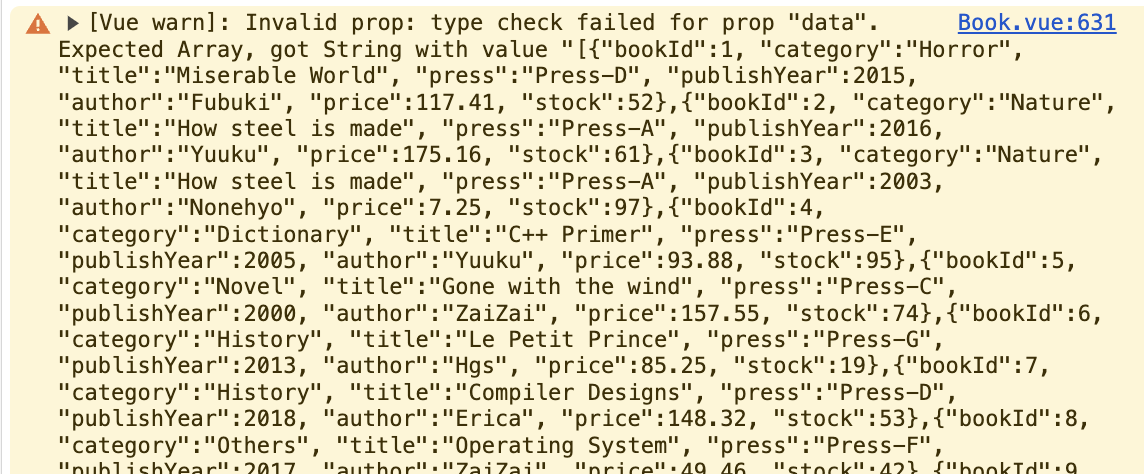
\includegraphics[width=0.9\textwidth]{attack-json-warning.png}
    \caption{Vue 数据错误警告}
    \label{fig:vue}
    \end{subfigure}%
    \begin{subfigure}{0.5\linewidth}
    \centering
    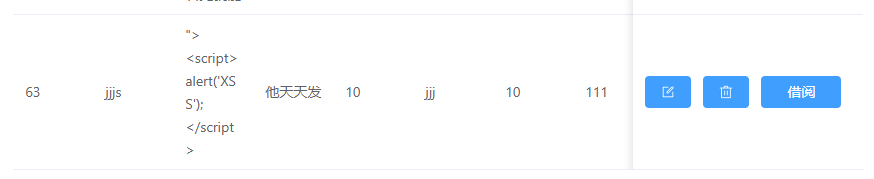
\includegraphics[width=0.9\textwidth]{attack-fin.png}
    \caption{正确显示注入数据}
    \end{subfigure}
    \caption{警告和解决成功图示}
\end{figure}

\section{502 Bad Gateway}

我们并没有约定这个错误码的含义,所以是网络通信的问题。

这个问题一般是在 Java 后端在请求处理时抛出异常,没有回复,Nginx 等待超时后自动中断并回复 502。查看 Nginx 日志可以了解问题细节,并给予针对性的修复。

\begin{figure}[!h]
    \centering
    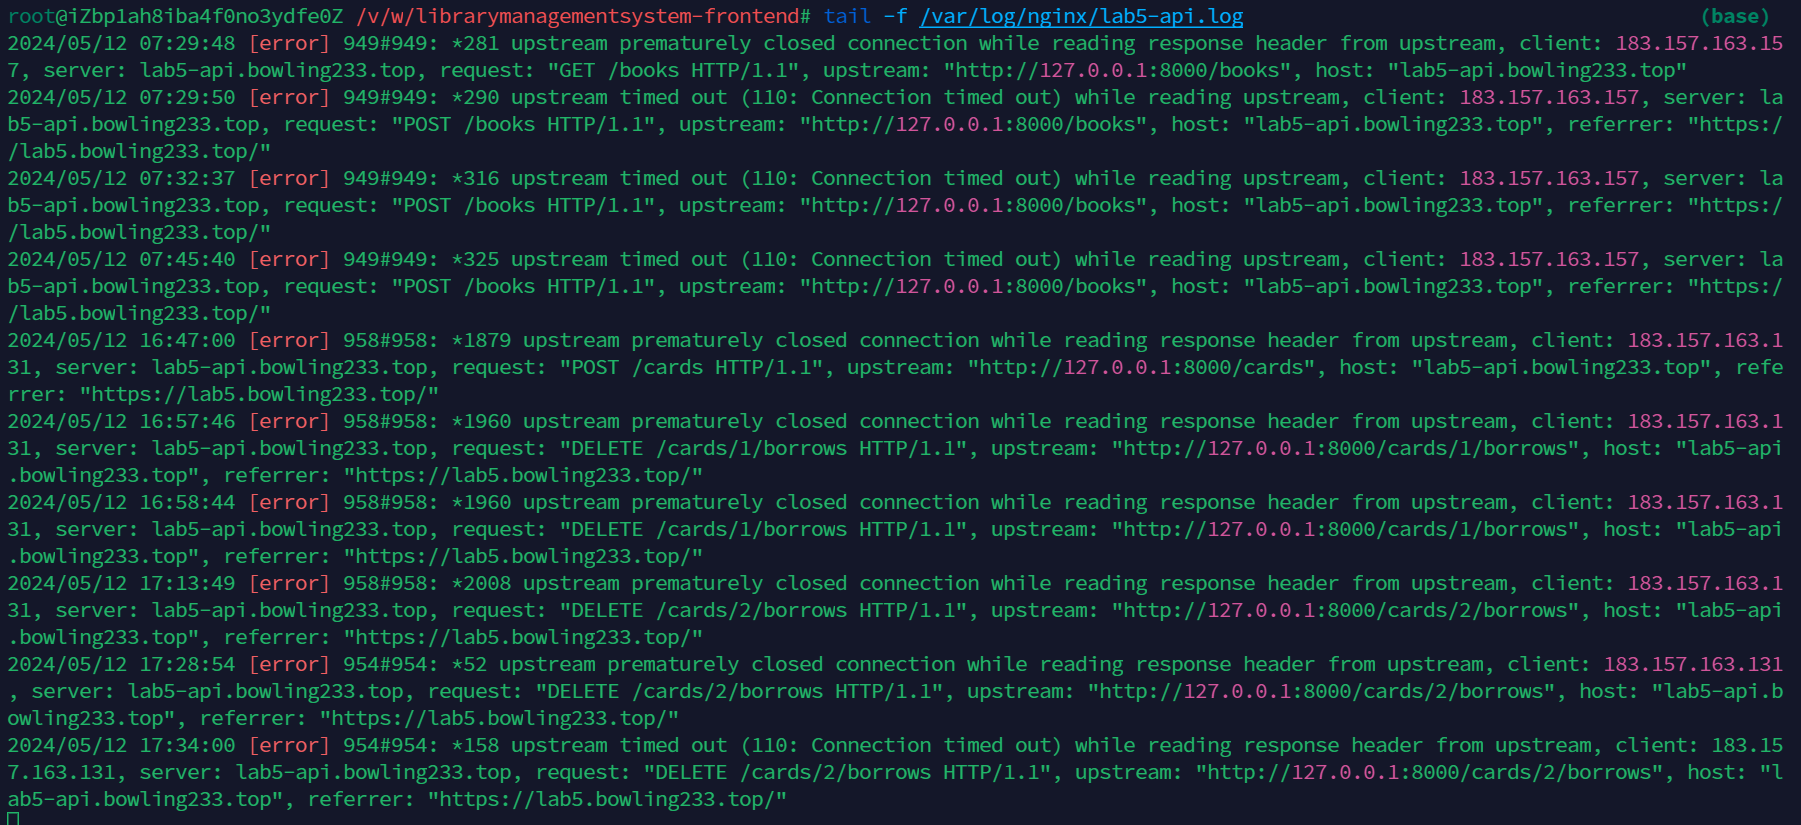
\includegraphics[width=\textwidth]{nginx.png}
    \caption{502 Bad Gateway 的相关日志}
    \label{fig:502}
\end{figure}

\chapter{思考题}

E-R 图、注入攻击、隔离级别均已在前文介绍和提及,这里不再赘述。作为超算队运维,我负责队内分布式集群管理,因此对思考题中针对电商系统中的高并发活动通常采取的措施更有兴趣。

查阅资料,可以了解到一般有以下措施:

\begin{itemize}
    \item 限流控制:通过限制每秒钟的请求次数或者并发连接数,来控制系统的访问量,防止系统被过多的请求压垮。
    \item 队列处理:将请求放入队列中逐个处理,保证每个请求按顺序执行,避免并发访问导致的竞争条件。
    \item 缓存优化:合理利用缓存技术,减轻数据库的压力,提高系统的响应速度。
    \item 分布式架构:采用分布式架构,将负载分散到多个服务器上,提高系统的承载能力。
    \item 数据库优化:针对热点数据进行优化,减少数据库的访问压力,提高系统的并发处理能力。
\end{itemize}

这其中用到的数据库其实远不止 MySQL 这种关系型数据库,还有 Redis 这种 KV 作为缓存,MongoDB 这种文档型数据库做收集。我们不仅要掌握好课内的关系型数据库,还应当多关注工业界新型存储技术、数据处理技术的发展。

在分布式集群运维中,我们也面临着相似的问题:集群每台机器的日志->分析器->数据库,其中分析器和数据库都需要解决高并发问题。目前我们采用 Elastic Stack,在分析器前加消息队列集群,数据库使用 Elastic 分布式集群。Elastic 作为文档型数据库,和课内学习的 MySQL 等关系型数据库不同,在分布式集群上的扩展性非常好,能够轻松处理海量数据。

\chapter{总结}

非常感谢助教gg本学期对 Lab 进行的更改,新的 Lab 前后端非常有意思,我身边做了的同学几乎都会在朋友圈晒一晒自己的成果,可以看出大家都从 Lab 中学到了很多。这次 Lab 的开发过程也让我对网络的知识得到了进一步实践,具备了构建、调试基础网络应用程序的能力。

\bibliography{report}

\end{document}